% !TeX spellcheck = pt_BR
\chapter{Estado da Arte}
\label{ch::arte}

\section{Introdução}
\label{sec::arte:intro}

A visualização computacional de funções é a base de muitas aplicações práticas em computação gráfica, tais como em videojogos e visualização molecular. O estudo destas funções permite igualmente outro tipo de cálculos, tais como colisões.

Para alcançar os objetivos propostos no presente projeto, é imperativo estudar os seguintes tópicos:

\begin{itemize}
	\item Funções implícitas;
	\item Técnicas de renderização em geral e algoritmos volumétricos em particular;
	\item Uso da \ac{API} \opengl e programação em \ac{GLSL}.
\end{itemize}


\section{Funções Implícitas}
\label{sec::arte:implicitas}

%\subsection{Definição e Aplicações}
%\label{ssec::arte:implicitas:def}

% O que é? Exemplo(s). Que aplicações têm?

Às funções definidas em função de uma variável dá-se o nome de \textbf{funções explícitas}. Exemplos clássicos em $\mathbb{R}^2$ incluem equações de retas ($y = mx + b$) e parábolas ($y = ax^2 + bx + c$). Ora, nem todos os subconjuntos de pontos no espaço cartesiano podem ser definidos por funções explícitas. Um exemplo comum em $\mathbb{R}^2$ é a circunferência (Figura \ref{fig::circumference}):

\begin{equation}
	(x - x_0)^2 + (y - y_0)^2 = r^2
	\label{eq::circ_implicita}
\end{equation}

onde $(x_0, y_0)$ é o centro e $r$ o raio.

\begin{figure}[!htbp]
	\centering
	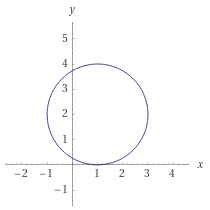
\includegraphics[scale=1.0]{circumference}
	\caption[Exemplo de uma circunferência]{Exemplo de uma circunferência de centro $(1, 2)$ e raio $2$.}
	\label{fig::circumference}
\end{figure}

Sendo uma equação de segundo grau, é possível representá-la através de duas funções explícitas:

\begin{eqnarray}
		y = y_0 + \sqrt{r^2 - (x - x_0)^2} \\
		y = y_0 - \sqrt{r^2 - (x - x_0)^2}
\end{eqnarray}

Esta transformação não é possível para todos os polinómios, em particular para graus superiores a $4$. Contudo, estas expressões polinomiais continuam a ser subconjuntos válidos de $\mathbb{R}^n$, necessitando então de formas alternativas de representação. Dois métodos e respetivas representações da circunferência são:

\begin{enumerate}
	\item \textbf{Funções paramétricas}: cada eixo é definido em ordem a uma variável adicional $t$:
	\begin{equation}
		\left\{\begin{array}{l}
			x = r\cos(t) \\
			y = r\sin(t)
		\end{array}\right.
	\label{eq::circ_parametrica}
	\end{equation}
	
	\item \textbf{Funções implícitas}: a equação não é definida a ordem a uma variável em particular (equação (\ref{eq::circ_implicita})).
\end{enumerate}

Uma \textbf{função implícita} é então definida por $f~:~\mathbb{R}^n \longrightarrow \mathbb{R}$, ou seja, para qualquer ponto em $\mathbb{R}^n$ é determinado um resultado em $\mathbb{R}$. Dependendo da função, o valor obtido pode ter significado, tal como uma grandeza física (\textit{e.g.} densidade de um líquido ou sua temperatura a cada ponto do espaço). Esta função diz-se \textbf{algébrica} caso seja polinomial em cada variável.

Por seu turno, em $\mathbb{R}^3$, a \textbf{iso-superfície} de uma função implícita é a superfície que satisfaz a condição $f(\mathbf{x}) = 0$ (onde, doravante, $\mathbf{x} \equiv (x,y,z)$). Esta pode ser suavizada através de um parâmetro $s \in \mathbb{R}$ tal que $f(\mathbf{x}) - s = 0$. Este efeito é utilizado diretamente e com sucesso nas Superfícies $\Pi$ \cite{Raposo2019}.


\todo{Mais aplicações.}


%\subsection{Desafios Computacionais}
%\label{ssec::arte:implicitas:desafios}


\section{Técnicas de Renderização: Visão Geral}
\label{sec::arte:render}

Muitos algoritmos de renderização têm vindo a ser investigados e usado em \textit{software} que implemente diversas técnicas para obter uma imagem final.\\


A nossa visão capta a luz refletida por objetos num determinado cenário. Durante o processo, a maioria dos comprimentos de onda das fontes de luz são absorvidos sendo o restante refletido. Como resultado final, os comprimentos de onda refletidos e captados pelos olhos constituem o que é interpretado como cor.

No entanto, o cálculo do percurso para cada partícula de luz num determinado cenário é na grande maioria dos casos algo impraticável devido à grande demora da obtenção dos resultados.

Por dito motivo, foram desenvolvidos métodos mais eficientes de cálculo da luz:
\begin{itemize}
    \item \textbf{Rasterização}, técnica ainda usada na pipeline do \opengl. Consiste na conversão numa imagem descrita geometricamente numa série de pixeis que quando juntos criam a imagem.
    
    \item \textbf{Ray Casting}, considera um cenário a ser observado por um determinado ponto de vista, o mesmo calcula a imagem observada baseado apenas na geometria e em leis óticas básicas.
    
    \item \textbf{Ray Tracing}, bastante próximo a como Ray Casting funciona, no entanto implementa também simulações ótica mais avançadas.
\end{itemize}

\hint{Breve introdução às categorias de técnicas/algoritmos de renderização.}\\
\revision{Categorização das técnicas.}


As funções implícitas representam simultaneamente uma grande oportunidade na área da computação gráfica e um enorme desafio. Se por um lado é possível obter a visualização de formas geométricas complexas com recurso a funções implícitas, por outro não há um método direto de determinar quais os pontos da iso-superfície.

Vários algoritmos têm sido propostos ao longo das últimas décadas, tais como \textit{marching cubes}\cite{Lorensen1987}, \textit{ray marching}, \textit{sphere tracing}\cite{Hart1996} e \textit{ray tracing}.

\begin{itemize}
	%\item \textbf{Rasterização}:\\
	%\hint{Técnica ainda utilizada na pipeline do OpenGL na fase final.}
	
	\item \textbf{Triangulação}:\\
	A iso-superfície é dividida em triângulos, os quais formam a \textit{mesh} a ser renderizada pela \ac{GPU}. Um exemplo é o algoritmo de \textit{Marching Cubes}\cite{Lorensen1987} no qual o espaço é dividido em cubos onde o valor da função implícita é calculado para cada vértice. A análise dos sinais permite determinar quais arestas do cubo a superfície interseta, num total de 256 possíveis combinações de triângulos.
	
	\item \textbf{\textit{Ray Tracing} e algoritmos volumétricos}:\\
    
	
	\item \hint{Mais técnicas/algoritmos?}
\end{itemize}


\section{\emph{Ray Marching}}
\label{sec::arte:raymarch}

\hint{Como funciona o algoritmo? É paralelizável? Se sim, como e porquê?}

\textit{Ray marching} é uma simples técnica que tal como no tradicional \textit{ray tracing}, não é tão simples de resolver uma superfície (ou até impossível caso sem o uso de métodos numéricos interativos). Em \textit{ray tracing} apenas nos focamos na interseção do raio emitido com a superfície, enquanto no algoritmo de \textit{ray marching} marchamos na direção tomada até encontrarmos uma interseção (isto se a mesma existir).\\

Isto é nos interessante caso:
\begin{itemize}
    \item precisemos de renderizar volumes que não são uniformes;
    \item renderizemos funções implícitas ou fractais;
    \item tenhamos interesse em renderizar outros tipos de funções paramétricas onde a interseção não é conhecida antecipadamente, como \textit{parallel mapping};
\end{itemize}

\todo{Imagem de exemplo algoritmo naive em 2D}\\

\subsection{Sphere Tracing}
\textit{Sphere tracing} é um possível algoritmo de \textit{ray marching}. No entanto, nem todos os usos de \textit{ray marching} beneficiam deste método, porque estes não conseguem ser convertidos para este esquema.

\textit{Sphere tracing} é usado para renderizar \textbf{superfícies implícitas}.
Visto que esta função pode ser resolvida para cada ponto, podemos ir em frente e estimar a maior esfera possível que possa caber no atual passo de marcha. Então sabemos que a próxima distancia a marchar é pelo menos tão grande quanto o raio da dita esfera. Desta forma adaptamos então o numero de passos a marchar e tornamos com o processo muito mais rápido.\\

\todo{Imagem de exemplo algoritmo spheretracing em 2D}\\

No entanto em \textit{sphere tracing} é um requisito saber calcular com antecipação a distância minima entre um dado ponto e a superfície em questão. Dão se a estas funções o nome de \textbf{\textit{Signed Distance Functions} (SDF)}.
O uso das mesmas torna impraticável a aplicação de \textit{sphere tracing} para funções implícitas. \\

\todo{Adicionar à lista de acronimos SDF: Signed Distance Functions}\\
\todo{Imagem de exemplo de uma SDF}\\




O algoritmo geral de \textit{ray marching} contempla os seguintes quatro passos:

\begin{enumerate}
	\item \textbf{\textit{Ray casting}}:
	
	\item \textbf{\textit{Sampling}}:
	
	\item \textbf{\textit{Shading}}:
	
	\item \textbf{\textit{Compositing}}:
\end{enumerate}


\section{\opengl}
\label{sec::arte:opengl}

\hint{Não recomendo um rip-off do meu relatório, mas ele pode servir de base para esta secção, tentando melhorá-lo e corrigir possíveis gafes.}


\section{Conclusões}
\label{sec::arte:conc}

\ldots Whiskas Saquetas.
